
\begin{center}
	\LARGE Med hjælpemidler
\end{center}
\begin{opgavetekst}{Opgave 1}
	En eksponentialfunktion $f$ er givet ved
	\begin{align*}
		f(x) = 7\cdot 1.3^x
	\end{align*}	
\end{opgavetekst}
\begin{delopgave}{}{1}
	Bestem begyndelsesværdien og fremskrivningsfaktoren for $f$.
\end{delopgave}
\begin{delopgave}{}{2}
	Bestem vækstraten for $f$ og brug denne til at bestemme, hvor mange procent $f$ øges med, hvis vi øger $x$ med 1.
\end{delopgave}	

\begin{opgavetekst}{Opgave 2}
	Bruttonationalproduktet (BNP) for et lille land er i år 2000 på $1300$ milliarder. Det antages, at 
	bruttonationalproduktet vokser med 5$\%$ om året. 
\end{opgavetekst}
\begin{delopgave}{}{1}
	Opstil en eksponentialfunktion, der beskriver BNP for landet som funktion af antal forløbne år efter år 2000.
\end{delopgave}	
\begin{delopgave}{}{2}
	Bestem BNP efter 10 år
\end{delopgave}
\begin{delopgave}{}{3}
	I hvilket årstal vil BNP for landet være på 2000 mia.?
\end{delopgave}

\begin{opgavetekst}{Opgave 3}
	Grafen for to potensfunktioner $f$ og $g$ kan ses på Figur \ref{fig:potensgraf}.
	\begin{figure}[H]
		\centering
		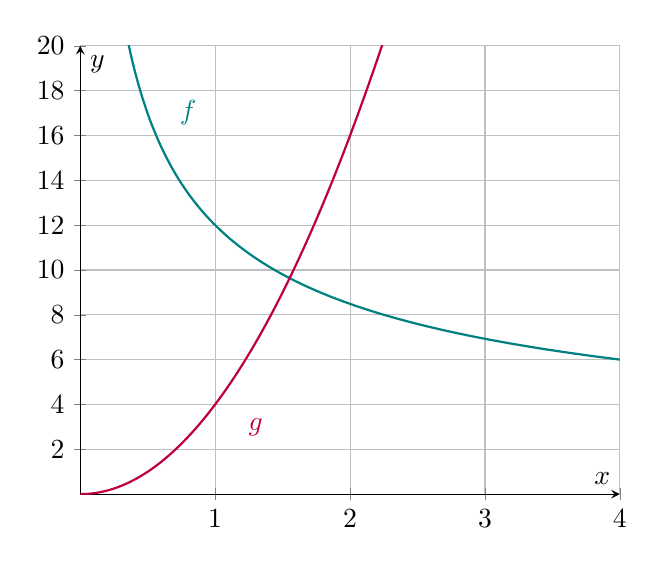
\begin{tikzpicture}
			\begin{axis}[
				axis lines = middle, 
				xmin = 0, xmax = 4, 
				ymin = 0, ymax = 20,
				grid = both, 
				ytick = {0,2,...,20},
				xlabel = $x$, ylabel = $y$
				]
				\addplot[thick, color = teal, domain = 0.2:6, samples = 200] {12*x^(-0.5)};
				\addplot[thick, color = purple, domain = 0:6, samples = 200] {4*x^(2)};
				\node[color = teal] at (axis cs: 0.8,17) {$f$};
				\node[color = purple] at (axis cs: 1.3,3) {$g$};
			\end{axis}
		\end{tikzpicture}
		\caption{Grafer for potensfunktionerne $f$ og $g$.}
		\label{fig:potensgraf}
	\end{figure}
	\phantom{h}
\end{opgavetekst}
\begin{delopgave}{}{1}
	Bestem $b$-værdien for $f$ og $g$.
\end{delopgave}
\begin{delopgave}{}{2}
	Bestem hvilke af følgende intervaller som $a$-værdierne for $f$ og $g$ tilhører.
	\begin{enumerate}[label=\roman*)]
		\item $a < 0$,
		\item $0 < a < 1$,
		\item $1 < a$.
	\end{enumerate}
\end{delopgave}
\begin{delopgave}{}{3}
	Brug Figur \ref{fig:potensgraf} til at løse ligningen $g(x) = 16$.
\end{delopgave}

\begin{opgavetekst}{Opgave 4}
	Det antages, at \href{https://github.com/ChristianJLex/TeachingNotes/raw/master/2023-2024/Data%20og%20lign/PotensData.xlsx}{\color{blue!60} dette datasæt} kan beskrives ved en potenssammenhæng $f$.
\end{opgavetekst}
\begin{delopgave}{}{1}
	Lav potensregression på tallene fra datasættet og bestem en forskrift for $f$.
\end{delopgave}
\begin{delopgave}{}{2}
	Bestem $f(2)$.
\end{delopgave}
\begin{delopgave}{}{3}
	Løs ligningen $f(x) = 5$.
\end{delopgave}

\begin{opgavetekst}{Opgave 5}
	Antallet af bakterier i en opløsning kan beskrives ved eksponentialfunktionen
	\begin{align*}
		f(x) = 2.1\cdot 1.07^x,
	\end{align*}
	hvor $f$ er antal bakterier i mia og $x$ er antal forløbne døgn.
\end{opgavetekst}
\begin{delopgave}{}{1}
	Afgør, om $f$ er voksende eller aftagende.
\end{delopgave}
\begin{delopgave}{}{2}
	Bestem fordobling/halveringskonstanten for $f$.
\end{delopgave}

\begin{opgavetekst}{Opgave 6}
	Grafen for en potensfunktion $g$ skærer gennem punkterne $(2,3)$ og $(5,10)$. 
\end{opgavetekst}
\begin{delopgave}{}{1}
	Bestem forskriften for $g$.
\end{delopgave}	
\begin{delopgave}{}{2}
	Tegn grafen for $g$ på intervallet $[0,6]$.
\end{delopgave}	
\begin{meretekst}
	En anden potensfunktion $h$ har forskriften
	\begin{align*}
		h(x) = 7\cdot x^{-0.3}.
	\end{align*}
\end{meretekst}
\begin{delopgave}{}{3}
	Bestem skæringspunktet mellem grafen for $g$ og grafen for $h$. 
\end{delopgave}
	